\documentclass[t]{beamer}
\usetheme{Copenhagen}
\setbeamertemplate{headline}{} % remove toc from headers
\beamertemplatenavigationsymbolsempty

\usepackage{amsmath, array, tikz, bm, pgfplots, tcolorbox, graphicx, venndiagram, color, colortbl, xfrac}
\pgfplotsset{compat = 1.16}
\usepgfplotslibrary{statistics}
\usetikzlibrary{calc}

\title{Hypothesis Testing}
\subtitle{Single Sample Mean}
\author{}
\date{}

\AtBeginSection[]
{
  \begin{frame}
    \frametitle{Objectives}
    \tableofcontents[currentsection]
  \end{frame}
}

\begin{document}

\pgfmathdeclarefunction{gauss}{2}{%
  \pgfmathparse{1/(#2*sqrt(2*pi))*exp(-((x-#1)^2)/(2*#2^2))}%
}

\begin{frame} 
\maketitle
\end{frame}

\begin{frame}
Student's $t$ distribution
Degrees of Freedom: $n-1$ --> As deg. of freedom grow, t distribution becomes more normal.
$t = \frac{\overline{x}-\mu}{\sigma/\sqrt{n}}$
\begin{center}
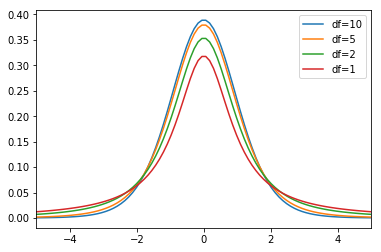
\includegraphics[scale=0.8]{../Images/t_distribution_df.png}
\end{center}
\end{frame}

* Can use $t$ distribution for smaller sample sizes ($n < 30$), as well as when $\sigma$ is unknown. 

* Do Python Code

* Example 1 - test statistic
* Example 2 - p-value
* Example 3 - confidence interval

\end{document}